\chapter{Uncertainty and Error Propagation}\label{chap:uncertainty}

Robots are systems that combine sensing, actuation, computation, and communication. All of its sub-systems are subject to a high degree
of uncertainty. This can be observed in daily life: phone calls with poor signal make it hard to understand the other party,
text characters are difficult to read from far away or at low resolution, the wheels of your car may slip when accelerating on a rainy road from a red light, or when your neural network mistakes a cat for a dog. In robotics, measurements
taken by on-board sensors are sensitive to changing environmental conditions and subject to electrical and mechanical limitations.
Similarly, actuators are not accurate as joints and gears have backlash and wheels can slip. Finally, wireless communication in particular,
whether via radio or infrared, is notoriously unreliable. Consider how these types of
uncertainty are all different: are they continuous or discrete? How does the uncertainty corrupt the ``ideal?'' How can these various
types of uncertainties be quantified and accounted for? So far, we have considered uncertainty only as far as limitations in accuracy and precision, but assumed that they do not matter. The goals of this chapter are to understand:
\begin{itemize}
    \item how to treat uncertainty mathematically using probability theory,
    \item how measurements with different uncertainty can be combined,
    \item and how error propagates when taking multiple measurements in a row.
\end{itemize}

This will help us to better understand how sensor error affects higher level features and decisions, but also create the basis for dealing with uncertainty and the problems that arise from it. 

This chapter requires an understanding of random variables, probability density functions, and the Normal
(alternatively called the ``Gaussian'') distribution. These concepts are explained in a robotic sensing context in Appendix~\ref{sec:pdfs}.

\section{Uncertainty in Robotics as Random Variable}

As quantities such as ``distance to a wall,'' ``position on the plane,'' or ``I can see a blue cross (yes/no)'' are uncertain, we can
consider them random variables. A \textsl{random variable}\index{Random Variable} can be thought of as the outcome of a ``random''
experiment, such as the face shown when rolling a die, or the speed of an individual molecule of gas in a room. Just because a
variable is random does not mean we know nothing about it. For instance, we can roll a fair six-sided die hundreds of times
and create a table of likelihoods of each side coming up. We can also measure the temperature in a room and understand the
average speed of those gas molecules using the kinetic theory of gases.

Experiments in robotics rarely involve true statistical randomness due to their scale and design. Instead, there are two primary sources
of uncertainty: sensors and physical interactions. Sensors are intrinsically noisy due to the physical phenomena associated with them.
These sources of uncertainty are often modelled using Gaussian (or ``Normal'') probability distribution functions, as they accurately model measurement uncertainty at large samples, per the Central Limit Theorem. Moreover, Gaussian distributions are mathematically convenient for combining multiple noisy measurements and analyzing propagation of uncertainty. 
% As such, we will assume here that random variables exhibit Gaussian probability distribution functions.
% As such, we will frequently assume that random variables here exhibit
As individual sensor readings can be considered random variables, quantities derived from multiple sensors can be considered random variables as well. Also, some physical interactions are very challenging to model accurately, especially those involving
friction, leading to uncertainty in the resulting models. This chapter focuses on how to characterize the uncertainty
of such aggregated quantities from the uncertainty that characterizes the individual sensors and modeling assumptions.

\section{Error Propagation}\label{sec:errorprop}
We'll begin with an example of error propagation that is a core motivation for needing to quantify uncertainty: the distance traveled by a
differential wheel robot given the rotations of its wheels. It turns out that the Gaussian Distribution is very appropriate to model the uncertainty in this process. The robot moves with an expected displacement (e.g.\ as commanded by the motors on each wheel) plus some uncertain displacement that can be decomposed into the radial and tangential directions for each timestep as a result of wheel slip; see \cref{fig:errorprop_odometry} for a diagram of this. We can say that \textsl{process noise} drawn from a Gaussian distribution was added to the position resulting from the commanded motion. This process noise has zero mean and distinct variance in both the radial and tangential directions; the process noise is a static property of the wheel-ground interaction.

Such a robot (when subject to slip) will actually increase the uncertainty in its position the farther it drives. Initially at a known location, the expected value (or mean) of its position will become increasingly uncertain, corresponding to an increasing position variance. This variance is obviously somehow related to the variance of the underlying mechanism (the process variance), namely the slipping wheel. Interestingly, we will see its position variance grow much faster orthogonal to the robot's direction of motion, as small errors in orientation have a much larger cumulative effect on position than small errors in the longitudinal direction. This is illustrated in \cref{fig:errorprop_odometry}.

\begin{figure}
	\centering
	% 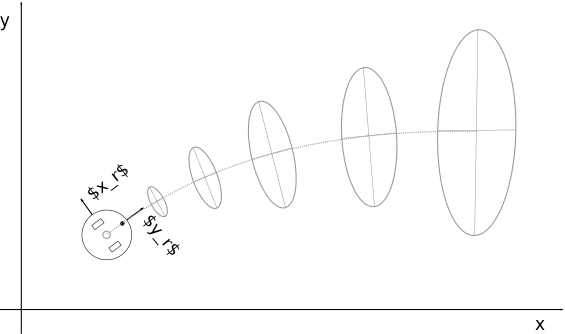
\includegraphics[width=\textwidth]{figs/errorprop_odometry}
    \def\svgwidth{\textwidth}
    \import{./figs/}{errorprop_odometry.pdf_tex}
	\caption{Two-dimensional Normal distribution depicting growing uncertainty as the robot moves. Albeit starting with equal
    uncertainty in $x$ and $y$, the large effect of small errors in orientation causes the error to grow faster in $y$-direction of the robot.}
	\label{fig:errorprop_odometry}
\end{figure}

If only there were a way to correct this unbounded error with some sort of sensor measurement! However, even these sensor measurements would be affected by uncertainty, so we will have to take this into account as well. We'll come up with a correction that is able to accommodate this shortly.

Similarly, when estimating distance and angle to a wall from point cloud data, the uncertainty of the random variables describing distance and angle to the wall are related to the uncertainty of \textsl{each} point measured on the wall. These relationships are formally captured by the \textsl{error propagation law}\index{Error Propagation Law}.

The key intuition behind the error propagation law is that the variance of each component that contributes noise to a random variable has a weight associated with it. This weight is a function of how strongly that component influences the random variable. Measurements that have little effect on the
aggregated random variable should also have little effect on its variance and vice versa. ``How strongly'' one variable affects another
can be expressed by the ratio of how small changes of the first variable relate to small changes in the second one. This concept should sound familiar, as it is none other 
than the partial derivative of the first variable with respect to the second. For example, let $y=f(x)$ be a function that maps a random variable $x$ (a sensor reading) to a random variable $y$ (a feature). Let the standard deviation of $x$ be given by $\sigma_x$. We can then calculate the resulting standard deviation $\sigma_y$ by
\begin{equation}
\sigma_y=\left(\frac{\partial f}{\partial x}\right) \sigma_x
\end{equation}
and its variance $\sigma_y^2$ as
\begin{equation}
\sigma_y^2=\left(\frac{\partial f}{\partial x}\right)^2 \sigma_x^2
\end{equation}
In case $\mathbf{y}=f(\mathbf{x})$ is a multivariable function that maps $n$ inputs to $m$ outputs, variances between these
variables may be represented by \textsl{covariance matrices}\index{Covariance Matrix}, a representation of the various combinations in
which these variables may affect one another, one by one. A covariance matrix holds the variance of each $n$ input variables along its diagonal and is zero otherwise, if the random variables are not correlated. We can then write
\begin{equation}
\Sigma^Y= J \Sigma^X J^T ,
\end{equation}
where $\Sigma^X$ and $\Sigma^Y$ are the $n \times n$ and $m \times m$ covariance matrices holding the variances of the input and output variables respectively, and
$J$ is a $m \times n$ \textsl{Jacobian} matrix, which holds the partial derivatives $\frac{\partial f_i}{\partial x_j}$. As $J$ has $n$ columns, each row contains partial derivatives with respect to $x_1$ to $x_n$.

\subsection{Example: Line Fitting}\label{sec:linefitting}
Detecting walls is a fairly common sensing task for a mobile robot, and can be accomplished with a range-bearing sensor like a  LIDAR. We can make some simplifying assumptions for the sake of this next example, namely that a wall sensed by a 2D spinning LIDAR would appear as a straight line of points in 3D space. Thus, our wall detection problem can be described as estimating the angle $\alpha$ and distance $r$ of a line (the wall) from a set of points (LIDAR readings) given by $(\rho_i,\theta_i)$ using \cref{eq:linealpha,eq:liner}. We can now express the relationship of changes of $ \rho_i$ to changes in $ \alpha$ by
\begin{equation}
\frac{\partial \alpha}{\partial \rho_i} .
\end{equation}
Similarly, we can calculate $ \frac{\partial \alpha}{\partial \theta_i}$, $ \frac{\partial r}{\partial \rho_i}$ and $ \frac{\partial r}{\partial \theta_i}$. We can do this because we have derived analytical expressions for $ \alpha$ and $ r$ as a function of $ \theta_i$ and $ \rho_i$ in \cref{chap:feature_extraction}.

We are now interested in deriving equations for calculating the variance of $ \alpha$ and $ r$ as a function of the variances of the distance measurements. Let's assume each distance measurement $ \rho_i$ has variance $ \sigma^2_{\rho,i}$ and each angular measurement $ \theta_i$ has variance $ \sigma^2_{\theta,i}$. We now want to calculate $ \sigma^2_{\alpha,i}$ as the weighted sum of  $ \sigma^2_{\rho,i}$ and $ \sigma^2_{\theta,i}$, each weighted by its influence on $ \alpha$:

\begin{equation}
    \sigma_{\alpha,i}^2 = \frac{\partial \alpha_i}{\partial \rho_i}^2 \sigma_{\rho,i}^2 + \frac{\partial \alpha_i}{\partial \theta_i}^2 \sigma_{\theta,i}^2 .
\end{equation} 

Derivation of $\sigma_{r,i}^2$ is done similarly.

% In matrix form, 
% \begin{equation}
%     % \Sigma_i^2 
%     % =
%     \left[
%         \begin{array}{c}
%             \sigma_{\alpha,i}^2 \\ 
%             \sigma_{r,i}^2
%         \end{array}
%     \right]
%     =
%     % \left[
%     %     \begin{array}{cc}
%     %     \end{array}
%     % \right]^2

%     \left[
%         \begin{array}{c}
%             \sigma_{\rho,i}^2 \\ 
%             \sigma_{\theta,i}^2
%         \end{array}
%     \right] .
% \end{equation}

More generally, if we have $ I$ input variables $ X_i$ and $K$ output variables $Y_k$, the covariance matrix of the output variables $ \sigma_Y$ can be expressed as $\sigma_Y^2=\frac{\partial f}{\partial X}^2 \sigma_X^2$ where $\sigma_X$ is the covariance matrix of input variables and $J$ is a Jacobian matrix of a function $ f$ that calculates $Y$ from $X$ and has the form

\begin{equation}
J=
\frac{\partial \bf{f}}{\partial \bf{X}}
=\left[
\begin{array}{ccc}
  \frac{\partial f_1}{\partial X_1} & \ldots & \frac{\partial f_1}{\partial X_I}\\
  \vdots & \ddots & \vdots\\
  \frac{\partial f_K}{\partial X_1} & \ldots & \frac{\partial f_K}{\partial X_I}
 \end{array}
 \right] .
\end{equation}

% In the line fitting example, $ J$ would contain the partial derivatives of $ \alpha$ with respect to all $ \rho_i$ ($i$-entries) followed by the partial derivatives of $ \alpha$ with respect to all $ \theta_i$ in the first row. In the second row, $ J$ would hold the partial derivatives of $ r$ with respect to $ \rho_i$ followed by the partial derivatives of $ r$ with respect to $ \theta_i$. 
% As there are two output variables, $ \alpha$ and $ r$, and $2I$ input variables (each measurement consists of an angle and distance), $ J$ is a 2 $\times$ (2$I$) matrix.
% The result is therefore a 2$\times$2 covariance matrix that holds the variances of $ \alpha$ and $ r$ on its diagonal.

\subsection{Example: Odometry}
\screencast{https://www.youtube.com/watch?v=ubg_AAM7Zd8}{errorpropagation}
Whereas the line fitting example demonstrated a many-to-one mapping (where multiple instantaneous measurements form a feature), odometry requires calculating the variance that results from multiple sequential measurements.  Error propagation allows us to not only express the robot's position, but also the variance of this estimate. Our list of questions to answer for this task is as follows:
\begin{enumerate}
\item What are the input variables and what are the output variables?
\item What are the functions that calculate output given an input?
\item What is the variance of the input variables?
\end{enumerate}

As usual, we describe the robot's position by a tuple $ (x,y,\theta)$. These are the three output variables. We can measure the distance each wheel travels $ \Delta s_r$ and $ \Delta s_l$ based on the encoder ticks and the known wheel radius. These are the two input variables. We can now calculate the change in the robot's position by calculating
\begin{eqnarray}
\Delta s &=& \frac{\Delta s_r + \Delta s_l}{2}\\
\Delta x  &=& \Delta s~\text{cos}(\theta)\\
\Delta y  &=& \Delta s~\text{sin}(\theta)\\
\Delta \theta &=& \frac{\Delta s_r-\Delta s_l}{b}
\end{eqnarray}

The robot's new position is then given by
\begin{equation}
f(x,y,\theta,\Delta s_r, \Delta s_l)=[x,y,\theta]^T + [\Delta x, \Delta y, \Delta \theta]^T
\end{equation}
We now have a function that relates our measurements to our output variables. What makes things complicated here is that the output variables are also a function of their previous values. Therefore, their variance does not only depend on the variance of the input variables, but also on the previous variance of the output variables. We therefore need to write
\begin{equation}\label{eq:errorpropodom}
\Sigma_{p'}=\nabla_p f \Sigma_p \nabla_p f^T + \nabla_{\Delta_{r,l}}f \Sigma_{\Delta}\nabla_{\Delta_{r,l}}f^T .
\end{equation}
The first term is the error propagation from an initial position $ p=[x,y,\theta]$ to a new position $ p'$. For this we need to calculate the partial derivatives of $ f$ with respect to x, y and $ \theta$. This is a 3x3 matrix:
\begin{equation}
\nabla_p f=\left[\frac{\partial f}{\partial x} \quad \frac{\partial f}{\partial y} \quad \frac{\partial f}{\partial \theta}\right]=\left[\begin{array}{ccc}1 &\quad 0 &\quad -\Delta s~\text{sin}(\theta +\Delta \theta /2)\\0 &\quad 1 &\quad \Delta s~\text{cos}(\theta + \Delta \theta/2)\\0 &\quad 0 &\quad 1\end{array}\right] .
\end{equation}
The second term is the error propagation of the actual wheel slip. This requires calculating the partial derivatives of $ f$ with respect to $ \Delta s_r$ and $ \Delta s_l$, which is a 3x2 matrix. The first column contains the partial derivatives of $ x,y,\theta$ with respect to $ \Delta s_r$. The second column contains the partial derivatives of $ x,y,\theta$ with respect to $ \Delta s_l$:
\begin{scriptsize}
\begin{equation}
\nabla_{\Delta_{r,l}} f=\left[
\begin{array}{ccc}
\frac{1}{2}\cos(\theta+\frac{\Delta \theta/2}{b})
-\frac{\Delta s}{2b}\sin(\theta+\frac{\Delta \theta}{b})
& \quad & \frac{1}{2}\cos(\theta+\frac{\Delta \theta/2}{b})
-\frac{\Delta s}{2b}\sin(\theta+\frac{\Delta \theta}{b})
\\
\frac{1}{2}\sin(\theta+\frac{\Delta \theta/2}{b})
+\frac{\Delta s}{2b}\cos(\theta+\frac{\Delta \theta}{b})
& \quad & \frac{1}{2}\sin(\theta+\frac{\Delta \theta/2}{b})
+\frac{\Delta s}{2b}\cos(\theta+\frac{\Delta \theta}{b})
\\
\frac{1}{2} & \quad & -\frac{1}{2}
\end{array}
\right] .
\end{equation}
\end{scriptsize}

Finally, we need to define the covariance matrix for the measurement noise. As the error is proportional to the distance traveled, we can define $ \Sigma_{\Delta}$ by
\begin{equation}
\Sigma_{\Delta}=\left[\begin{array}{cc}k_r|\Delta s_r| & 0\\0 & k_l|\Delta s_l|\end{array}\right] .
\end{equation}
Here $ k_r$ and $ k_l$ are constants that need to be found experimentally and $ |\cdot |$ indicates the absolute value of the distance traveled. We also assume that the error of the two wheels is independent, which is expressed by the zeros in the matrix.

We now have all ingredients for Equation~\ref{eq:errorpropodom}, allowing us to calculate the covariance matrix of the robot's pose just as in \cref{fig:errorprop_odometry}.




%The goals of this section are:

%\begin{itemize}
%\item to introduce a technique known as the Kalman filter to %perform action and perception updates exclusively using Gaussian %distributions.
%\item to formally introduce the notion of a feature map.
%\item to develop an example that puts everything we learned so far together: forward kinematics, error propagation, and sensor noise.
%\end{itemize}

\section{Optimal Sensor Fusion}
%The Kalman filter is an optimal way to fuse observations that follow a Gaussian distribution. Just like the Bayes filter, the Kalman filter has a prediction step and an update step. The prediction step uses a  model of the system (such as the forward kinematics of your robot, sometimes called a motion model) and the update step uses a sensor model (such as the error distribution calibrated from its sensors). The Kalman filter does not only update the state of the system (the robot's position) but also its variance (representing uncertainty). For this, it requires knowledge of all of the variances involved in the system (e.g., wheel-slip and sensor error) and uses them to weigh each measurement accordingly. Before providing the equations for the Kalman filter, we will make use of a simple example that explains what ``optimal'' means in this context.


We have now seen how errors from \emph{different} sources can propagate into error of compound measurements by means of the equations that relate input to output error. We are now interested in how independent observations of the \emph{same} quantity can be combined. For example, we have considered measurements obtained from two different wheels that are combined in a pose estimate. What about a case in which we receive two independent measurements of the robot's pose? Similarly, we have seen how to combine multiple point measurements into a line. How about two observations of the same line (distance and angle) from two different sensors? 

Let $ \hat{q_1}$ and $ \hat{q_2}$ be two different estimates of a random variable and $ \sigma^2_1$ and $ \sigma^2_2$ their variances, respectively. Let $ q$ be the true value. This could represent the true pose of a line, with observations having different variances when they are obtained by different means, say using a LIDAR for $ \hat{q_1}$ and by using a camera for $ \hat{q_2}$. We can now define the weighted mean-square error
 \begin{equation}
S=\displaystyle\sum_{i=1}^{n}\frac{1}{\sigma_i} (q-\hat{q_i})^2 .
\end{equation}
That is, $ S$ is the sum of the errors of each observation $ \hat{q_i}$ with $n=2$, weighted by the inverse of their standard deviation $ \frac{1}{\sigma_i}$. 

Each error is weighted  with the inverse of its standard deviation to put more emphasis on observations whose uncertainty is low. Minimizing  $S$ by talking the derivatives of $S$ with respect to $\hat{q}_i$ and setting them to zero, yields the following optimal expression for $q$:
\begin{equation}
q=\frac{\hat{q_1}\sigma_2^2}{\sigma_1^2+\sigma_2^2}+\frac{\hat{q_2}\sigma_1^2}{\sigma_1^2+\sigma_2^2}
\end{equation}
or, equivalently,
\begin{equation}
q=\hat{q_1}+\frac{\sigma_1^2}{\sigma_1^2+\sigma_2^2}(\hat{q_2}-\hat{q_1})\label{eq:optimalfusion}
\end{equation}

We have now derived an expression for fusing two independent observations with different variances that provably minimizes the error between our estimate and the real value. As $q$ is a linear combination of two random variables (Section~\ref{sec:lcombrandom}), the new variance is given by
\begin{equation}
\sigma^2=\frac{1}{\frac{1}{\sigma_1^2}+\frac{1}{\sigma_2^2}} .
\end{equation}
Interestingly, the resulting variance is smaller than both $\sigma_1$ and $\sigma_2$; that is, incorporating additional observations can always help improve accuracy instead of introducing more uncertainty.

\subsection{The Kalman Filter}
\screencast{https://youtu.be/IFeCIbljreY}{kalmanfilter}
Although we have introduced the problem above as fusing two observations of the same quantity and weighting them by their variance, we can also interpret the equation above as an update step that calculates a new estimate of an observation based on its old estimate and a new measurement. Specifically, we can interpret the expression $\hat{q_2}-\hat{q_1}$ from \cref{{eq:optimalfusion}} as the difference between what the robot actually sees and what it thinks it should see. This term is known as \textsl{innovation}\index{Innovation} in what is also known as the \emph{Kalman filter}\index{Kalman filter}. We can now
rewrite (\ref{eq:optimalfusion}) from above into
\begin{equation}
\hat{x}_{k+1}=\hat{x}_k+K_{k+1}\tilde{y}_{k+1} \label{eq:kalmanperceptionstep},
\end{equation}
also known as the \emph{perception update step}\index{Perception step (Kalman filter)}.
Here, $ \hat{x}_k$ is the state we are interested in at time $ k$, $ K_{k+1}=\frac{\sigma_1^2}{\sigma_1^2+\sigma_2^2}$ is what is known as the \emph{Kalman gain}\index{Kalman gain}, and $ \tilde{y}_{k+1}=\hat{q_2}-\hat{q_1}$  as the innovation.

Unfortunately, there are few systems that allow us to directly measure the information we are interested in. Rather, we obtain a sensor measurement $ z_k$ that we need to convert into something we can use to update our state. We can then consider the inverse problem of predicting your measurement $ z_k$ from your state $ x_k$. This is done using the observation model $ H_k$, so that
\begin{equation}
\tilde{y}_{k}=z_k-H_k x_k ,
\end{equation}
where 
% $y_k$ is the innovation, 
% $z_k$ is the latest measurement, and 
$H_kx_k$ is the measurement prediction.
In our example, $ H_k$ was just the identity matrix; in a robot position estimation problem, $ H_k$ is a function that would predict how a robot would observe a shift in position through a sensor. As you can see, all the weighting based on variances is done in the Kalman gain $ K$.

% The \emph{perception update step} shown in \eqref{eq:kalmanperceptionstep} is only half of what the Kalman filter does - the other being the \emph{prediction update step}\index{Prediction step (Kalman filter)} which will be discussed later. The perception update step is exactly the same as we learned during error propagation. 

It is now time for a brief disclaimer: the Kalman filter only works for linear systems. Forward kinematics of even the simplest robots are mostly intrinsically non-linear, and so are observation models that relate sensor observations to the robot position. Non-linear systems can be dealt with by using the \textsl{Extended Kalman Filter}, which will be introduced a bit later on in the context of robot localization. %which linearizes both the process model and sensor model around the current state by using a first-order Taylor expansion.


\section{Take-home lessons}
\begin{itemize}
\item Uncertainty can be expressed by means of a probability density function.
\item More often than not, the Gaussian distribution is chosen as it allows treating error with powerful analytical tools.
\item In order to calculate the uncertainty of a variable that is derived from a series of measurements, we need to calculate a weighted sum in which each measurement's variance is weighted by its impact on the output variable. This impact is expressed by the partial derivative of the function relating input to output.
\item It is also possible to fuse independent observations, each with their own variance, of the same quantity. This will usually reduce the variance of the resulting observation. 
\end{itemize}

\section*{Exercises}\small
\begin{enumerate}
\item Given two observations $\hat{q}_1$ and $\hat{q}_2$ with variances $\sigma_1$ and $\sigma_2$ of a normal distributed process with actual value $\hat{q}$, an optimal estimate can be calculated by minimizing the expression
\begin{equation}
\nonumber
S=\frac{1}{\sigma_1^2}(\hat{q}-\hat{q}_1)^2+\frac{1}{\sigma_2^2}(\hat{q}-\hat{q}_2)^2
\end{equation}
Calculate $\hat{q}$ so that $S$ is minimized.
\item An ultrasound sensor measures distance $x=c\Delta t/2$. Here, $c$ is the speed of sound and $\Delta t$ is the difference in time between emitting and receiving a signal.
\begin{enumerate}
\item Let the variance of your time measurement $\Delta t$ be $\sigma_t^2$. What can you say about the variance of $x$, when $c$ is assumed to be constant? Hint: how does a change in $\Delta t$ affect $x$?
\item Now assume that $c$ is changing depending on location, weather, etc.\ and can be estimated with variance $\sigma_c^2$. What is the variance of $x$ now?
\end{enumerate}
\item Consider a unicycle that turns with angular velocity $\dot{\phi}$ and has radius $r$. Its speed is thus a function of $\dot{\phi}$ and $r$ and is given by
\begin{equation}
\nonumber
v=f(\dot{\phi},r)=r\dot{\phi}
\end{equation}
Assume that your measurement of $\dot{\phi}$ is noisy and has a standard deviation $\sigma_{\dot{\phi}}$.  Use the error propagation law to calculate the resulting variance of your speed estimate $\sigma_v^2$.
\item Consider a scenario in which a robot can localize itself against landmarks. Describe what happens to the robot's positional error in the following three cases:
\begin{enumerate}
\item the landmark location is known and the robot can reliably localize to it,
\item the landmark location has a variance and the robot can reliably localize to it,
\item both the landmark and localization mechanism have a variance.
\end{enumerate}
\item Write a program that graphically illustrates merging observations with two different variances in 1D and 2D.
\end{enumerate}
\normalsize
